\documentclass[10pt]{article}
\usepackage{icmlko}

\icmlmeta{IP 파운데이션 월드모델}{58}{다섯 배 반}{쉰여덟 개 노트 동안 순위 상관으로만 말했다 --- 그것이 기획서 앞에서 무엇을 뜻하는지 처음으로 옮긴다}

\begin{document}

\twocolumn[
\icmlheader

\begin{abstract}
노트 33부터 57까지 성능을 $\rho$로만 적었다. $+$0.35가 좋은지 나쁜지는 다른
$\rho$와 비교해서만 말했고, 팝업 기획서를 앞에 둔 사람에게 그것이 무엇을 뜻하는지
한 번도 옮기지 않았다. 옮긴다. 팝업 75건의 라벨은 log$_{10}$(일평균 방문자)이고
평균이 443명이다. 다른 다섯 도메인 --- 아이돌 · 게임 · 도서 · 펀딩 · 웹툰 ---
에서만 배우고 \textbf{팝업 라벨은 한 번도 보지 않은} 예측으로 75건을 다섯
분위로 나누면, \textbf{1분위 860명, 5분위 157명으로 5.5배 차이가 난다.}
예측 상위 20\%가 실제 상위 20\%를 맞히는 비율이 33\%다(무작위 20\%). 출처별로
거의 같다 --- 아이돌 $+$0.476, 펀딩 $+$0.473, 도서 $+$0.450, 게임 $+$0.445,
웹툰 $+$0.415. 노트 33의 ``출처 선택은 무의미하다''가 제품 수준에서 확인된다.
어느 시장에서 배우든 팝업 앞에서는 비슷하게 쓸모 있다. \textbf{한계도 같은
언어로 적어야 한다} --- 이것은 \emph{순위}이고 절대 방문자 수가 아니다. 눈금은
대상 도메인 8--20건을 재서 맞춰야 하며(노트 26 · 32) 그 절차는 여기 들어 있지
않다. 그리고 75건은 적다.
\end{abstract}
]

\section{$\rho$를 사람 말로}

노트 43에서 판정 기준을 스피어만 순위 상관으로 옮긴 뒤 쉰여덟 노트 동안 그것으로만
말했다. $+$0.3506이 $+$0.3440보다 낫다는 식이다. 그 숫자가 기획서를 앞에 둔
사람에게 무엇을 뜻하는지는 적은 적이 없다.

\begin{table}[t]
\centering\tsize
\caption{팝업 도메인.}
\begin{tabular}{lr}
\toprule
레코드 & 75건 \\
라벨 & log$_{10}$(일평균 방문자) \\
평균 & 2.65 (443명) \\
표준편차 & 0.56 ($\times\div$3.6) \\
\bottomrule
\end{tabular}
\end{table}

예측은 다섯 도메인에서 각각 배운 것의 평균이다. \textbf{팝업 라벨은 학습에도
정렬에도 쓰이지 않는다} --- 축만 보고, 다른 시장의 라벨로 배운 계수를 옮긴다.

\section{5.5배}

\begin{figure}[t]
\centering
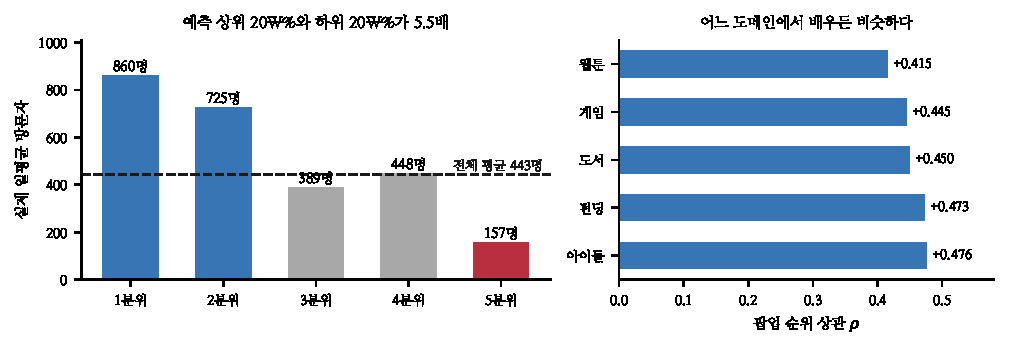
\includegraphics[width=\textwidth]{figs/product.pdf}
\caption{왼쪽 --- 예측 분위별 실제 방문자. 오른쪽 --- 출처별 순위 상관.}
\end{figure}

\begin{table}[t]
\centering\tsize
\caption{예측 다섯 분위. 각 15건.}
\begin{tabular}{lr}
\toprule
예측 분위 & 실제 일평균 방문자 \\
\midrule
1분위 (상위 20\%) & \textbf{860명} \\
2분위 & 725명 \\
3분위 & 389명 \\
4분위 & 448명 \\
5분위 (하위 20\%) & \textbf{157명} \\
\midrule
전체 평균 & 443명 \\
\bottomrule
\end{tabular}
\end{table}

\claimx{팝업 라벨을 전혀 쓰지 않고 기획서 축만으로, 예측 상위 20\%와 하위
20\%의 실제 방문자가 5.5배 차이 난다(860명 대 157명). 상위 20\% 적중률은
33\%로 무작위(20\%)의 1.7배다.}{3분위(389명)와 4분위(448명)가 뒤집혀 있다.
분위별 15건이라 요동이 크고, 중간 구간은 사실상 구분하지 못한다고 읽어야 한다.}

양 끝은 잘 가르고 가운데는 못 가른다. 실무에서는 그것으로 충분한 경우가 많다
--- 어느 기획을 밀지 고를 때 필요한 것은 순서지 정확한 방문자 수가 아니다.

\section{어느 시장에서 배우든 비슷하다}

\begin{table}[t]
\centering\tsize
\caption{출처별 팝업 예측.}
\begin{tabular}{lrr}
\toprule
출처 & $\rho$ & 상위 20\% 적중 \\
\midrule
아이돌 & $+$0.476 & 33\% \\
펀딩 & $+$0.473 & 33\% \\
도서 & $+$0.450 & 40\% \\
게임 & $+$0.445 & 40\% \\
웹툰 & $+$0.415 & 27\% \\
\midrule
다섯 평균 & $+$0.471 & 33\% \\
\bottomrule
\end{tabular}
\end{table}

폭이 $+$0.415에서 $+$0.476으로 좁다. \textbf{노트 33의 ``출처 선택은 무의미하다''가
제품 수준에서 확인된다} --- 아이돌 초동에서 배우든 크라우드펀딩 후원자 수에서
배우든 팝업 앞에서는 비슷하게 쓸모 있다. 다섯을 평균 내도 최고 하나와 같다.

이것이 이 방향의 원래 가설이기도 했다. 서로 다른 시장의 반응이 같은 축 위에서
같은 방향으로 움직인다면, 어느 시장의 데이터든 다른 시장을 예측하는 데 쓸 수
있다. 여섯 도메인 2,181건에서 그렇게 보인다.

\section{같은 언어로 적는 한계}

\begin{itemize}[leftmargin=1.1em,itemsep=0.2em]
\item \textbf{순위지 방문자 수가 아니다.} 예측값은 눈금이 없다. 절대 수를 내려면
      대상 도메인 8--20건을 재서 중심과 산포를 맞춰야 하고(노트 26 · 32), 그
      절차는 이 숫자에 들어 있지 않다.
\item \textbf{75건이다.} 분위마다 15건이라 3 · 4분위 역전 같은 것이 쉽게 나온다.
      귀무분포도 가장 넓다(노트 43).
\item \textbf{중간을 못 가른다.} 2--4분위가 725 · 389 · 448명으로 섞여 있다.
\item \textbf{팝업 축은 사람이 매긴다.} 노트 49에서 위키백과로 대체하려다
      실패했다. 새 기획을 넣으려면 사람이 다섯 축을 읽어야 한다.
\item \textbf{이 75건은 계수 검증을 통과한 것들이다.} 입장·참여 기준으로 세었고
      스코프가 확인된 레코드만 남겼다(노트 1--8). 그 필터를 통과하지 못한
      기획에 대해서는 아무 말도 하지 않는다.
\end{itemize}

\section{다음}

\begin{enumerate}[leftmargin=1.3em,itemsep=0.15em]
\item 눈금 보정을 이 파이프라인에 붙여 절대 방문자 수를 낸다. 노트 26 · 32의
      절차가 있고 여섯 도메인에서 다시 재지 않았다.
\item 웹툰 전체 수집 완료 후 전면 재측정(1,141/3,973 진행 중).
\item 팝업 표본 --- 75건이 모든 한계의 뿌리다.
\item 중간 분위를 가르는 것이 가능한지 --- 지금은 양 끝만 쓸 수 있다.
\end{enumerate}

\vspace{0.6em}
\hrule height 0.3pt
\vspace{0.5em}
{\footnotesize
\textbf{참고문헌}\\[0.3em]
Spearman, C. (1904). The proof and measurement of association between two things.
\emph{American Journal of Psychology}, 15(1), 72--101.\\[0.15em]
Ben-David, S. et al. (2010). A theory of learning from different domains.
\emph{Machine Learning}, 79(1--2), 151--175.\\[0.15em]
Schönemann, P. H. (1966). A generalized solution of the orthogonal Procrustes
problem. \emph{Psychometrika}, 31(1), 1--10.\\[0.15em]
Copas, J. B. (1983). Regression, prediction and shrinkage. \emph{JRSS B},
45(3), 311--354.\\[0.15em]
Salganik, M. J., Dodds, P. S., Watts, D. J. (2006). Experimental study of
inequality and unpredictability in an artificial cultural market.
\emph{Science}, 311(5762), 854--856.
}

\end{document}
